\documentclass[presentation]{beamer}
%\documentclass[handout,9pt]{beamer}

\mode<presentation>
{
%  \usetheme{Warsaw}
  % or ...
\usetheme{Goettingen}
%\usetheme{Hannover}

%\usecolortheme{crane}
%\usecolortheme{beaver}
%\usecolortheme{beetle}
%\usecolortheme{dolphin}
%\usecolortheme{whale}
%\usecolortheme{wolverine}
%\usecolortheme{albatross}
%  \setbeamercovered{transparent}
  % or whatever (possibly just delete it)
}


\setbeamertemplate{navigation symbols}{}

\usepackage[utf8]{inputenc}
\usepackage[spanish, es-tabla, es-nodecimaldot]{babel}

\usepackage{listings}
\usepackage{tikzsymbols}

%\usepackage{times}
%\usepackage[T1]{fontenc}
% Or whatever. Note that the encoding and the font should match. If T1
% does not look nice, try deleting the line with the fontenc.


\title[Mediciones temp.\\ Fibra Óptica \\ Pozos petroleros] % (optional, use only with long paper titles)
{Utilizando mediciones continuas de temperatura en pozos de hidrocarburos}

%\subtitle

\author[SP]
{G. Sebastián Pedersen\\
\small sebasped@gmail.com}%\inst{1}}
% - Give the names in the same order as the appear in the paper.
% - Use the \inst{?} command only if the authors have different
%   affiliation.

\institute[] % (optional, but mostly needed)
{3er. Ciclo de Charlas de Matemática --- ICI --- UNGS 
%  \inst{1}%
%  Instituto de Industria\\
%  Universidad Nacional de General Sarmiento
%  \and
%  \inst{2}%
%  Department of Theoretical Philosophy\\
%  University of Elsewhere}
% - Use the \inst command only if there are several affiliations.
% - Keep it simple, no one is interested in your street address.
}

\date[] % (optional, should be abbreviation of conference name)
{Jue 03 de Octubre de 2019\\ 
%\vspace{.5cm}
%{
%\small\url{subir_la_charla_a_github_y_poner_la_url}
}



% If you have a file called "university-logo-filename.xxx", where xxx
% is a graphic format that can be processed by latex or pdflatex,
% resp., then you can add a logo as follows:

% \pgfdeclareimage[height=0.5cm]{university-logo}{university-logo-filename}
% \logo{\pgfuseimage{university-logo}}


% Delete this, if you do not want the table of contents to pop up at
% the beginning of each subsection:
%\AtBeginSubsection[]
%{
%  \begin{frame}<beamer>{Outline}
%    \tableofcontents[currentsection,currentsubsection]
%  \end{frame}
%}


% If you wish to uncover everything in a step-wise fashion, uncomment
% the following command: 

%\beamerdefaultoverlayspecification{<+->}




\begin{document}

\begin{frame}
  \titlepage
  \vspace{-.5cm}
  \begin{abstract}
  	{La herramienta clásica en la industria petrolera para mediciones en pozo es el PLT (Production Logging Tool). En esta charla abordaremos qué pueden aportar las mediciones continuas de temperatura por fibra óptica en pozos de hidrocarburos.}
  \end{abstract}
  
\end{frame}


%Geoterma
%
%Medición FO, y equipo DTS
%
%Calor + transporte
%PDE
%
%Caso 1D
%
%Barrett
%
%Productores, inyectores
%
%Fases, presiones
%
%Convencional, no convencional
%
%Joule-Tomson
%
%Avance uniforme/parabólico. Inyectores polímero
%
%Conductividad térmica, capacidad calorífica
%
%Separador
%
%Dowstream / upstream
%
%Chowk managment
%
%
%1. Problema central a contar
%no olvidar de diferencia con PLT
%2. Contexto
%3. Modelado
%4. Resultados
%5. Referencias
%no olvidar subir la charla a github




%\newpage
\section{La cuestión central}

%\subsection{Expresiones}
\begin{frame}{¿Qué se quiere saber de un pozo de hidrocarburos y por qué?}
	\begin{block}{Determinar la dinámica del pozo:}
	\end{block}
	\begin{columns}
		\column{0.4\textwidth}
	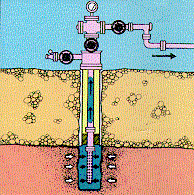
\includegraphics[width=\textwidth]{./pozo.png}
		
		\column{0.6\textwidth}
	\begin{itemize}
	\item Producción por capas:
	\begin{itemize}
		\item El total en superficie se sabe.
		\item Cuánto está saliendo para cada punzado (profundidad).
	\end{itemize}
	\item Variaciones temporales de la producción por capas:
		\begin{itemize}
%		\item 
		\item Coyuntural vs. histórico.
	\end{itemize}
	
	\item Relación con la zona: %prod pozos vecinos, nuevas perforaciones, cambios de fase en la producción, producción por yacimientos
		\begin{itemize}
			\item Prod. pozos vecinos.
			\item Nuevas perforaciones, otros yacimientos, cambios de fase, etc.
		\end{itemize}

	\end{itemize}
\end{columns}
\end{frame}


\section{Contexto y mediciones}
\begin{frame}{Para determinar la dinámica del pozo se realizan mediciones}
	\begin{block}{}
		Herramienta más popular: PLT (Production Logging Tool)
	\end{block} 
	\begin{columns}
	\column{0.5\textwidth}
	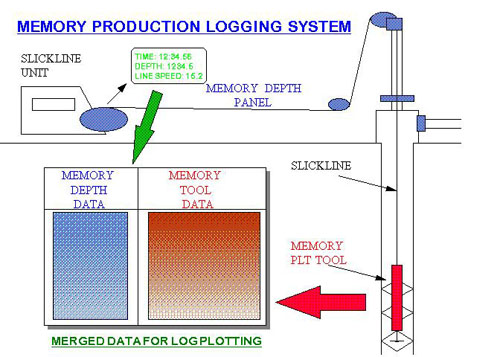
\includegraphics[scale=2, width=\textwidth]{./plt.png}
	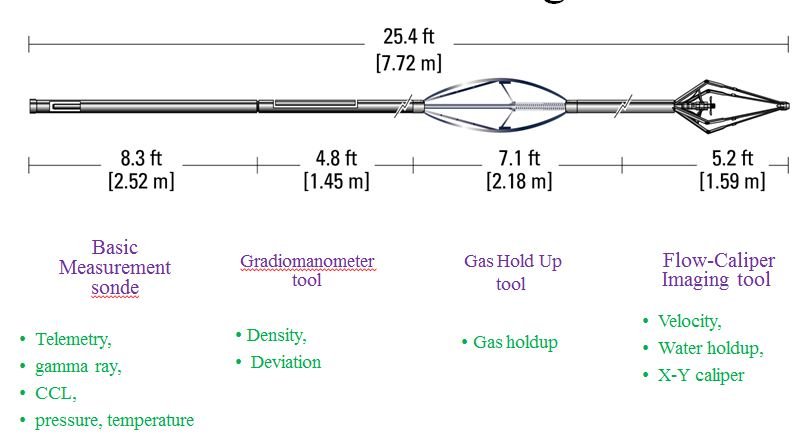
\includegraphics[scale=2, width=\textwidth]{./plt2.png}
	
	\column{0.6\textwidth}
	\begin{itemize}
		\item Pros:
		\begin{itemize}
			\item Herramienta aceptada en la industria.
			\item Mide caudales.
			\item Mide temperatura, presión.
			\item Se deducen varias cosas más: fases, densidad, etc.
		\end{itemize}
		\item Contras:
		\begin{itemize}
			\item Sus mediciones son ``fotos''. 
			\item Cada uso implica una intervención al pozo.
			\item Se accede a la información \emph{luego} de la medición.
			\item Algunas deducciones no son del todo confiables.
		\end{itemize}
%		\end{itemize}
		
	\end{itemize}
\end{columns}
\end{frame}



\begin{frame}{Resultado típico de medición con PLT}
%	\begin{block}{Herramienta más popular: PLT (Production Logging Tool)}
%	\end{block} 
	\begin{columns}
		\column{0.5\textwidth}
%		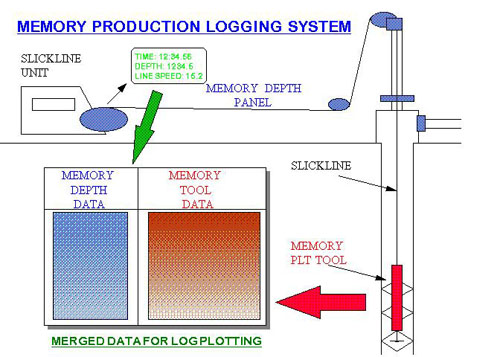
\includegraphics[scale=2, width=\textwidth]{./plt.png}
		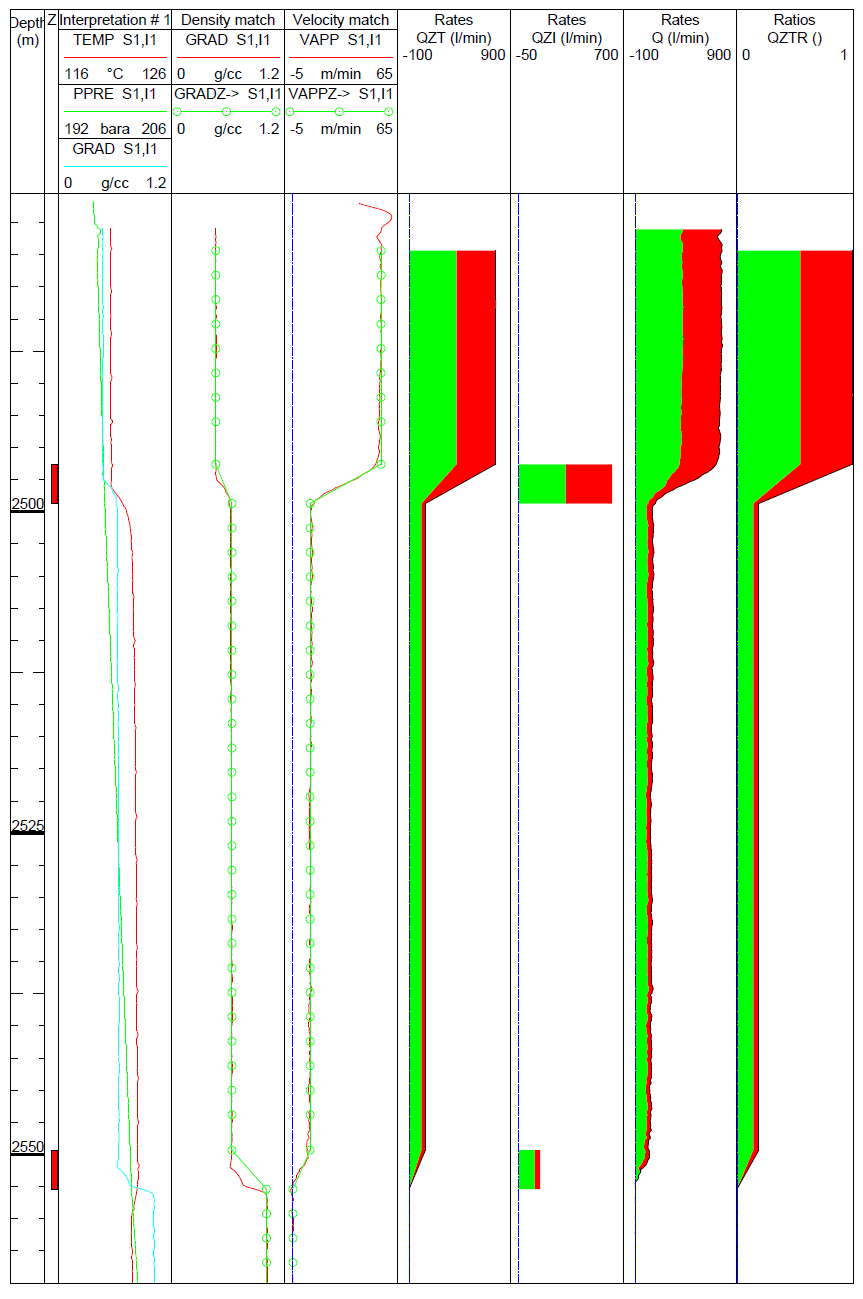
\includegraphics[scale=2, width=\textwidth]{./plt3.png}
		
		\column{0.5\textwidth}
		Para cada profundidad dentro del pozo:
		\begin{itemize}
			\item Temperatura.
			\item Presión.
			\item Densidades.
			\item Velocidad spinner.
			\item Caudales de cada fase (petróleo, gas, agua).
			\item Etc.
%			\begin{itemize}
%				\item Herramienta aceptada en la industria.
%				\item Mide caudales.
%				\item Mide temperatura, presión.
%				\item Se deducen varias cosas más: fases, densidad, etc.
%			\end{itemize}
%			\item Contras:
%			\begin{itemize}
%				\item Sus mediciones son ``fotos''. 
%				\item Cada uso implica una interveción al pozo.
%				\item Algunas deducciones no son del todo confiables.
%			\end{itemize}
%			%		\end{itemize}
%			
		\end{itemize}
	\end{columns}
\end{frame}



\begin{frame}{Para determinar la dinámica del pozo:}
	\begin{block}{Mediciones con fibra óptica (FO): DTS (Distributed Temperature Sensor)}
	\end{block} 
	\begin{columns}
		\column{0.4\textwidth}
		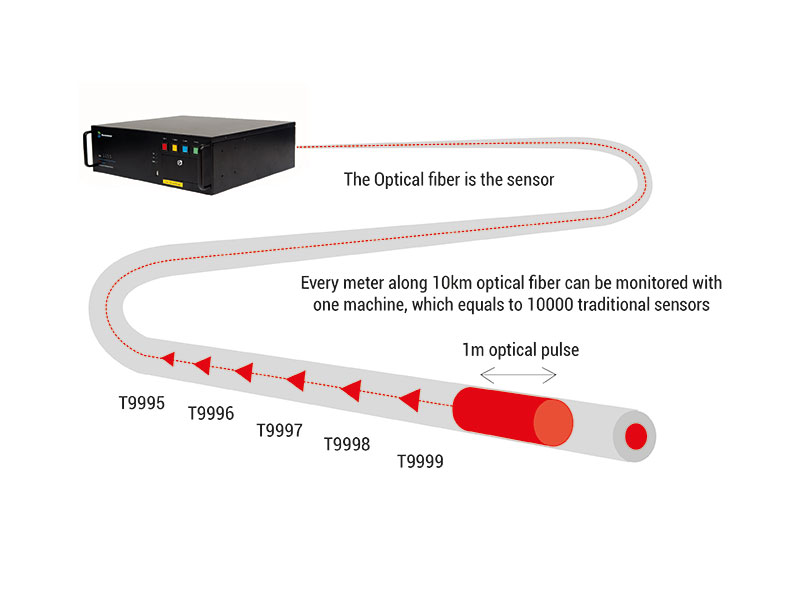
\includegraphics[scale=2, width=\textwidth]{./dts.png}
		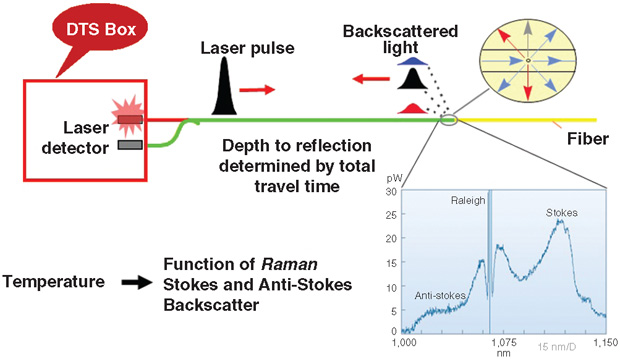
\includegraphics[scale=2, width=\textwidth]{./dts2.png}
		
		\column{0.6\textwidth}
		\begin{itemize}
			\item Pros:
			\begin{itemize}
				\item Se interviene una única vez el pozo.
				\item Queda midiendo y da información continua.
				\item Se accede a la información de la medición instantáneamente.
%				\item Mide temperatura, presión.
%				\item Se deducen varias cosas más: fases, densidad, etc.
			\end{itemize}
			\item Contras:
			\begin{itemize}
				\item Mide solamente temperatura. 
				\item Es una herramienta todavía algo ``nueva'' en la industria.
				\item Se hace necesario un trailer de medición cerca del pozo.
			\end{itemize}
			%		\end{itemize}
			
		\end{itemize}
	\end{columns}
\end{frame}



\section{Modelado e implementaciones}

\begin{frame}{¿Cómo se usa la temperatura para inferir la dinámica de un pozo?}
	\begin{block}{El efecto de la geoterma:}
		La temperatura de la Tierra más o menos aumenta 1 C por cada 30 m. de profundidad.
\end{block} 
%\begin{columns}
%	\column{0.4\textwidth}
	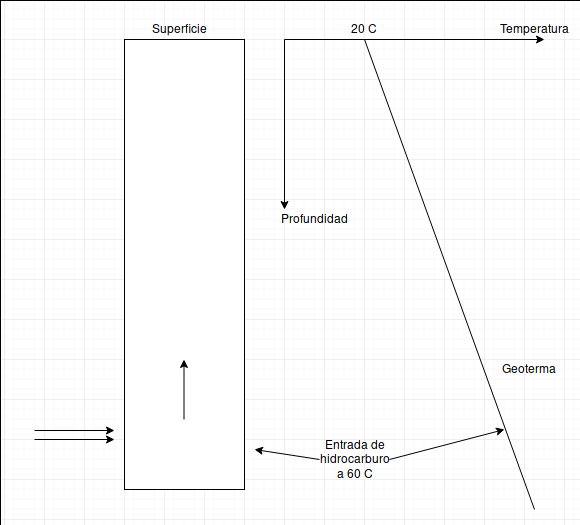
\includegraphics[height=.6\textheight]{./geoterma.png}
\end{frame}

\begin{frame}{¿Cómo se usa la temperatura para inferir la dinámica de un pozo?}
	\begin{block}{El efecto de la velocidad de subida del hidrocarburo:}
	Sube rápido y entonces se enfría poco.
\end{block} 
%\begin{columns}
%	\column{0.4\textwidth}
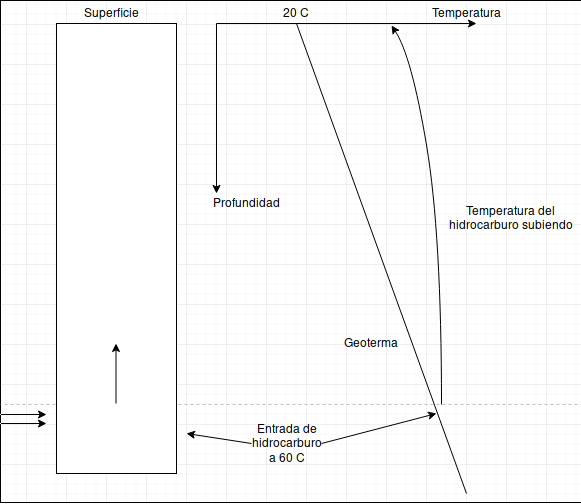
\includegraphics[height=.7\textheight]{./subiendo.png}
\end{frame}


\begin{frame}{¿Cómo se usa la temperatura para inferir la dinámica de un pozo?}
	\begin{block}{El efecto mezcla con otras capas productoras:}
		A diferentes profundidades el hidrocarburo entra al pozo a distinta temperatura, por el efecto de la geoterma.
	\end{block} 
	%\begin{columns}
	%	\column{0.4\textwidth}
	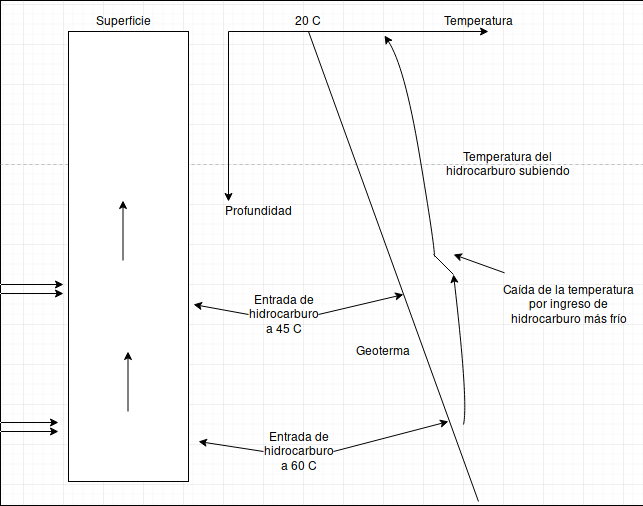
\includegraphics[height=.65\textheight]{./mezcla.png}
\end{frame}



\begin{frame}{¿Cómo se usa la temperatura para inferir la dinámica de un pozo?}
	\begin{block}{Conclusión:}
		La caída de temperatura depende del caudal que ingresa. 
	\end{block}
\begin{itemize}
	\item 1er. ingreso de caudal $Q_1$:
	\begin{itemize}
		\item La temp. $T$ cae lentamente por la geoterma.
	\end{itemize}
	\item 2do. ingreso de caudal $Q_2$
		\begin{itemize}
		\item La temp. $T$ cae abruptamente producto de la mezcla.
		\item La temp del caudal total $Q_1+Q_2$ cae lentamente por la geoterma.
	\end{itemize}
	\item Etc. para cada capa productora por donde ingresa hidrocarburo.	
\end{itemize}

\begin{block}{Modelo simplificado:}
	Tenemos una temperatura $T$ que depende de la profundidad y del caudal. 
\end{block}

	%\begin{columns}
	%	\column{0.4\textwidth}
%	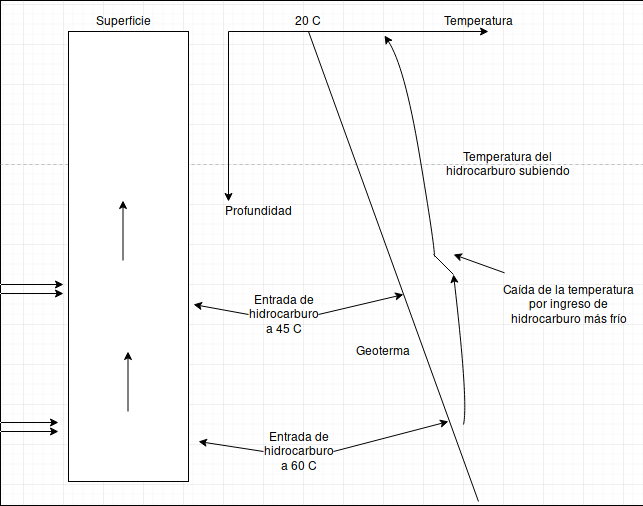
\includegraphics[height=.65\textheight]{./mezcla.png}
\end{frame}



\begin{frame}{¿Cómo se usa la temperatura para inferir la dinámica de un pozo?}
	\begin{block}{Modelo simplificado:}
		Tenemos una temperatura $T$ que depende de la profundidad y del caudal. 
	\end{block}

	\begin{columns}
	\column{0.65\textwidth}
	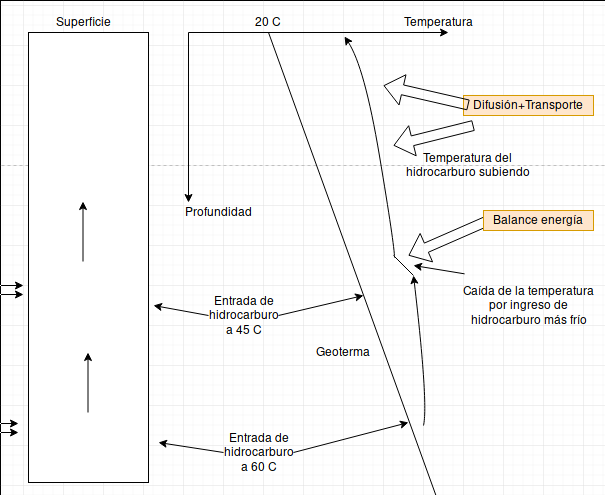
\includegraphics[width=\textwidth]{./modelo.png}
%	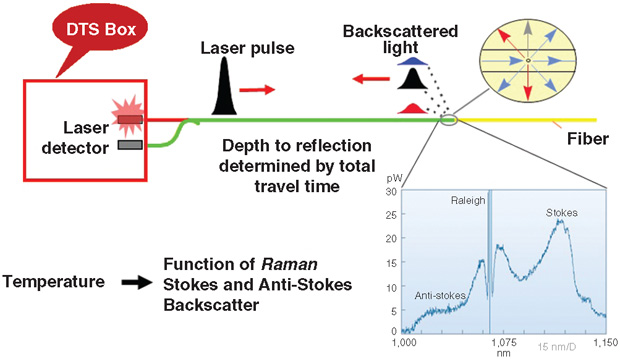
\includegraphics[scale=2, width=\textwidth]{./dts2.png}
	
	\column{0.45\textwidth}
La temperatura $T$ es afectada por:
\begin{itemize}
	\item Difusión de calor: del hidrocarburo contra la Tierra (geoterma).
	\item Transporte de calor: del hidrocarburo subiendo rápidamente.
	\item Balance de energía: mezcla con otra capa.
\end{itemize}
\end{columns}

\end{frame}




\begin{frame}{¿Cómo se usa la temperatura para inferir la dinámica de un pozo?}
	\begin{block}{El problema del Modelo:}
		\begin{itemize}
			\item Conocemos:
			\begin{itemize}
				\item La temperatura para cada profundidad: por el DTS con FO.
				\item El Caudal total en superficie
			\end{itemize}
			\item ¿Cómo averiguar el caudal entrante en cada capa?
		\end{itemize}
		¡Era la cuestión central original!
	\end{block}

	\begin{block}{La cuestión central reformulada:}
	\begin{itemize}
		\item Dados los caudales entrantes, podemos conocer la temperatura mediante calor+transporte
		\begin{itemize}
			\item Calor+transporte: es una ecuación diferencial a resolver.
			%			\item El Caudal total en superficie
		\end{itemize}
		\item Pero necesitamos el problema inverso: conocida la temperatura averiguar los caudales.
	\end{itemize}
\end{block}

\end{frame}
%	
%	\begin{columns}
%		\column{0.65\textwidth}
%		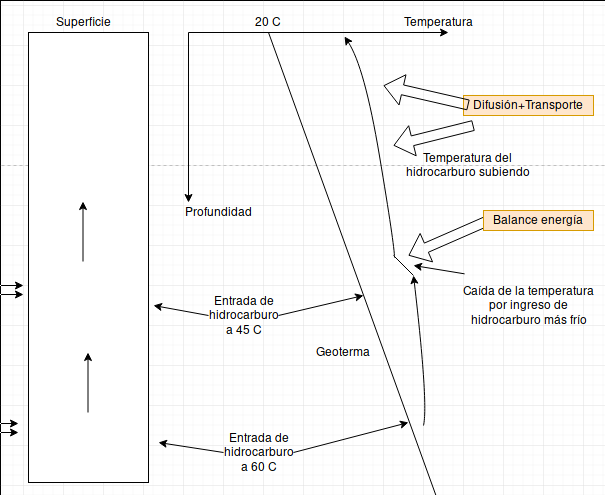
\includegraphics[width=\textwidth]{./modelo.png}
%		%	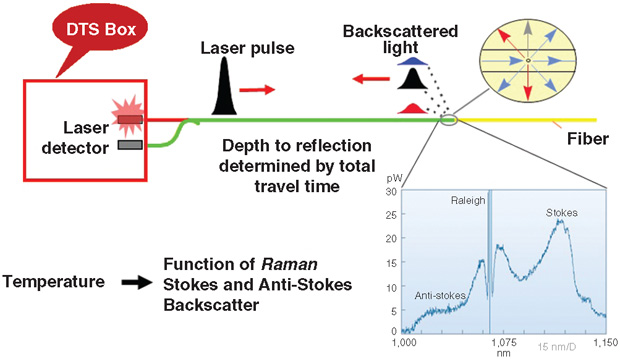
\includegraphics[scale=2, width=\textwidth]{./dts2.png}
%		
%		\column{0.45\textwidth}
%		La temperatura $T$ es afectada por:
%		\begin{itemize}
%			\item Difusión de calor: del hidrocarburo contra la Tierra (geoterma).
%			\item Transporte de calor: del hidrocarburo subiendo rápidamente.
%			\item Balance de energía: mezcla con otra capa.
%		\end{itemize}
%	\end{columns}

\begin{frame}{¿Cómo se usa la temperatura para inferir la dinámica de un pozo?}
	\begin{block}{La cuestión central reformulada:}
	\begin{itemize}
		\item Dados los caudales entrantes, podemos conocer la temperatura mediante calor+transporte
		\begin{itemize}
			\item Calor+transporte: es una ecuación diferencial, a resolver.
			\item $\rho c_p \frac{\partial T}{\partial t} - k \nabla^2 T + v\nabla T = 0 $ + condiciones de borde.
		\end{itemize}
		\item Pero necesitamos el problema inverso: conocida la temperatura averiguar los caudales.
	\end{itemize}
\end{block}


	\begin{block}{Idea para resolver el problema:}
	\begin{itemize}
		\item Ir variando los caudales entrantes en el modelo hasta pegarle a la temperatura medida por el DTS.
		\item Hay que resolver la ecuación diferencial cada vez.
	\end{itemize}
\end{block}


\end{frame}


%\begin{frame}{¿Cómo cambia la temperatura de un hidrocarburo en un pozo?}
%	IMAGEN y al lado
%	\begin{itemize}
%		\item Geoterma
%		\item velocidad
%		\item Difusión y transporte
%		\item mezcla con otras capas productoras
%		\item Joule-thomson
%		\item Cambios de fase
%	\end{itemize}
%\end{frame}


\section{Resultados}
\begin{frame}{Un resultado del modelo}
	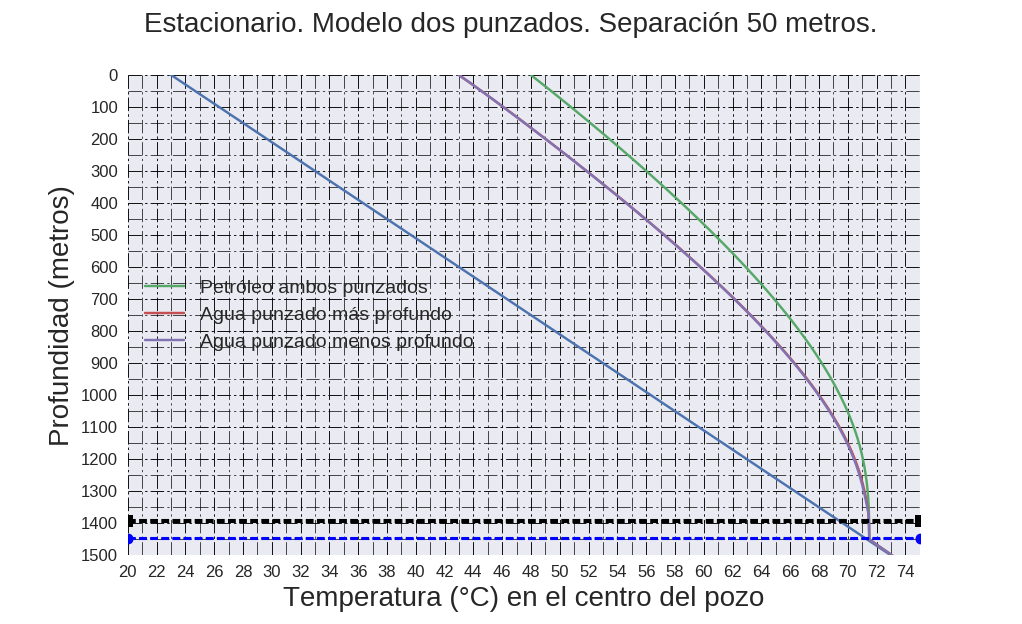
\includegraphics[height=.45\textheight]{./perfil2.png}
	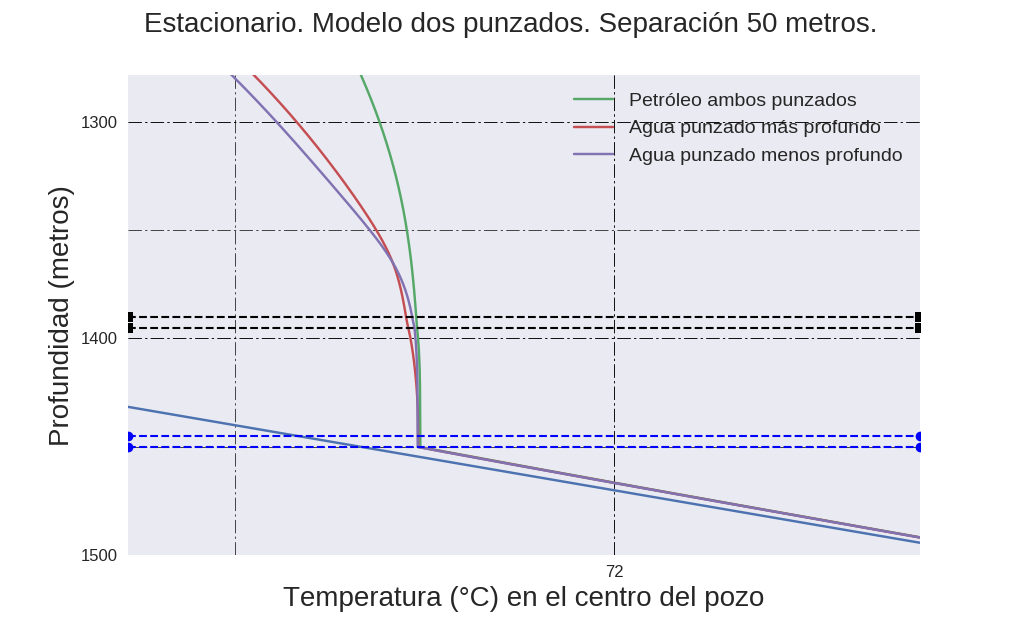
\includegraphics[height=.45\textheight]{./perfil1.png}
\end{frame}




\begin{frame}{Varios problemas}
	\begin{itemize}
		\item Resolver una ec. dif. es costoso:
		\begin{itemize}
			\item Elementos finitos con mucho poder de cálculo.
			\item O reducir dimensiones y simplificar a modelo menos confiable.
		\end{itemize}
		\item Para cada tiempo cambia el problema.
		\item Cambios de fase a medida que sube el hidrocarburo.
		\item Efecto Joule-Thomson.
		\item Parámetros del modelo difíciles de estimar:
		\begin{itemize}
			\item Conductividad térmica de los materiales.
			\item La capacidad calorífica de los materiales.
			\item Porosidad y permeabilidad.
		\end{itemize}
		\item Pozo convencional vs. \emph{no} convencional.
	\end{itemize}
%Separador
%Dowstream / upstream
%Chowk managment
\begin{block}{Problema aparte:}
	Análogo a pozos inyectores:
	\begin{itemize}
		\item Avance uniforme/parabólico. Inyectores polímero.
	\end{itemize}
\end{block}
\end{frame}




\section{Referencias}
\begin{frame}{Algunas referencias:}
	\begin{itemize}
		\item 
Fluid Flow and Heat Transfer in Wellbores, Rashid Hasan and Shah Kabir, SPE, 2002.
		\item The Essentials of Fiber-Optic Distributed Temperature Analysis, Schlumberger, 2019.
		\item Successful Flow Profiling of Gas Wells Using Distributed Temperature Sensing Data, Johnson. SPE 103097, 2006.
		\item Determining Gas Flow Rate and Formation Thermal Conductivity from Pressure and Temperature Profiles in Vertical Well, Barrett. SPE 152034, 2012.
		\item Wellbore Heat Transmission, Ramey, SPE 96, 1962.
		\item  The Estimation of Water Injection Profiles From Temperature Surveys, Nowak, 1953.
		\item Interpretation of Temperature Profiles in Water-Inyections Wells., Smith, 1975.
		
	\end{itemize}
	
\end{frame}
	
	
	
	
\section{}
\begin{frame}
	\textbf{\centering\LARGE{¡GRACIAS!}}
\end{frame}


\end{document}


